% This is the Reed College LaTeX thesis template. Most of the work 
% for the document class was done by Sam Noble (SN), as well as this
% template. Later comments etc. by Ben Salzberg (BTS). Additional
% restructuring and APA support by Jess Youngberg (JY).
% Your comments and suggestions are more than welcome; please email
% them to cus@reed.edu
%
% See http://web.reed.edu/cis/help/latex.html for help. There are a 
% great bunch of help pages there, with notes on
% getting started, bibtex, etc. Go there and read it if you're not
% already familiar with LaTeX.
%
% Any line that starts with a percent symbol is a comment. 
% They won't show up in the document, and are useful for notes 
% to yourself and explaining commands. 
% Commenting also removes a line from the document; 
% very handy for troubleshooting problems. -BTS

% As far as I know, this follows the requirements laid out in 
% the 2002-2003 Senior Handbook. Ask a librarian to check the 
% document before binding. -SN

%%
%% Preamble
%%
% \documentclass{<something>} must begin each LaTeX document
\documentclass[12pt,twoside]{reedthesis}
% Packages are extensions to the basic LaTeX functions. Whatever you
% want to typeset, there is probably a package out there for it.
% Chemistry (chemtex), screenplays, you name it.
% Check out CTAN to see: http://www.ctan.org/
%%
\usepackage{graphicx,latexsym} 
\usepackage{amssymb,amsthm,amsmath}
\usepackage{longtable,booktabs,setspace} 
\usepackage{chemarr} %% Useful for one reaction arrow, useless if you're not a chem major
\usepackage[hyphens]{url}
\usepackage{rotating}
\usepackage{natbib}
% Comment out the natbib line above and uncomment the following two lines to use the new 
% biblatex-chicago style, for Chicago A. Also make some changes at the end where the 
% bibliography is included. 
%\usepackage{biblatex-chicago}
%\bibliography{thesis}

% \usepackage{times} % other fonts are available like times, bookman, charter, palatino

\title{My Final College Paper}
\author{Gabriel Howland}
% The month and year that you submit your FINAL draft TO THE LIBRARY (May or December)
\date{May 2025}
\division{Mathematical and Natural Sciences}
\advisor{Peter Ksander}
%If you have two advisors for some reason, you can use the following
\altadvisor{Jim Fix}
%%% Remember to use the correct department!
\department{Computer Science and Theatre}
% if you're writing a thesis in an interdisciplinary major,
% uncomment the line below and change the text as appropriate.
% check the Senior Handbook if unsure.
%\thedivisionof{The Established Interdisciplinary Committee for}
% if you want the approval page to say "Approved for the Committee",
% uncomment the next line
\approvedforthe{Committee}

\setlength{\parskip}{0pt}
%%
%% End Preamble
%%
%% The fun begins:
\begin{document}

  \maketitle
  \frontmatter % this stuff will be roman-numbered
  \pagestyle{empty} % this removes page numbers from the frontmatter

% Acknowledgements (Acceptable American spelling) are optional
% So are Acknowledgments (proper English spelling)
    \chapter*{Acknowledgements}
	I want to thank a few people.

% The preface is optional
% To remove it, comment it out or delete it.
    \chapter*{Preface}
	This is an example of a thesis setup to use the reed thesis document class.
	
	

    \chapter*{List of Abbreviations}
		You can always change the way your abbreviations are formatted. Play around with it yourself, use tables, or come to CUS if you'd like to change the way it looks. You can also completely remove this chapter if you have no need for a list of abbreviations. Here is an example of what this could look like:

	\begin{table}[h]
	\centering % You could remove this to move table to the left
	\begin{tabular}{ll}
		\textbf{DMX}  	&  Digital Multiplex \\
		\textbf{sACN}  	&  Columbia Broadcasting System\\
		\textbf{Artnet}  	&  Center for Disease Control \\
		\textbf{CIA}  	&  Central Intelligence Agency\\
		\textbf{CLBR} 	&  Center for Life Beyond Reed\\
		\textbf{CUS}  	&  Computer User Services\\
		\textbf{FBI}  	&  Federal Bureau of Investigation\\
		\textbf{NBC}  	&  National Broadcasting Corporation\\
	\end{tabular}
	\end{table}
	

    \tableofcontents
% if you want a list of tables, optional
    \listoftables
% if you want a list of figures, also optional
    \listoffigures

% The abstract is not required if you're writing a creative thesis (but aren't they all?)
% If your abstract is longer than a page, there may be a formatting issue.
    \chapter*{Abstract}
	The preface pretty much says it all.
	
	\chapter*{Dedication}
	You can have a dedication here if you wish.

  \mainmatter % here the regular arabic numbering starts
  \pagestyle{fancyplain} % turns page numbering back on

%The \introduction command is provided as a convenience.
%if you want special chapter formatting, you'll probably want to avoid using it altogether

    \chapter*{Introduction}
         \addcontentsline{toc}{chapter}{Introduction}
	\chaptermark{Introduction}
	\markboth{Introduction}{Introduction}
	% The three lines above are to make sure that the headers are right, that the intro gets included in the table of contents, and that it doesn't get numbered 1 so that chapter one is 1.

% Double spacing: if you want to double space, or one and a half 
% space, uncomment one of the following lines. You can go back to 
% single spacing with the \singlespacing command.
%\onehalfspacing
 \doublespacing
	
This thesis explores lighting control, specifically for live performance. It will take a look at how lighting was originally controlled manually, how the technology has advanced to today through the use of time coding, and proposes a system for control that is reactive to a performer. Lighting control has advanced at a breakneck speed over the past half-century as the world entered a digital age. Where lighting control rooms were packed with levers and room-scale dimming racks now sit lighting desks, or even just a laptop. As the technology for controlling lights has advanced, the lighting design for live performances has gotten more complicated, while being largely prerecorded. Thus, while a designer's vision is accomplished in collaboration with the director and performers, it stays static barring catastrophe, which introduces interesting problems. Consider the actor who moves in tandem to a moving light. This is usually accomplished through hours of rehearsal, and fine-tuning movements in order to keep pace with the light. However, if the actor in a particular showing wanted to modify a movement, either in the route or in the speed, they would be constrained by the lighting.

%ADD SOME SHIT ABOUT APPIA HERE AND LIVENESS AND HOW ITS GOOD FOR PERFORMERS

    This thesis attempts to aleviate those constraints by creating a lighting control scheme that tracks a performer through a theatrical space. It is a reactive scheme that hopes to meet a few criteria: 1) The scheme must be lightweight; 2) The scheme must be able to run using off-the-shelf components and computing resources; 3) The scheme must be open source; 4) The scheme should run on top of existing theater infrastructure. It is worth mentioning that this concept is not revolutionary. There are numerous choices for high-end performer tracking offered by the likes of Cast Group's BLACKTRAX, Follow-Me, and zactrack. However, these systems are often closed-source, prohibitively expensive, hardware intensive, or otherwise difficult for small productions to access. The software developed during this thesis hopes to try to make it easier to access, which is why the scheme has criteria. 
    
    % probs cant use this line: "With this project comes deep research into the history of performance technology, namely how lighting control technology advanced over the previous ~50 years, and see how the changes affected what lighting meant for the stage."
    
    This thesis is spread across three(?) chapters. The first is a literature review of the theory and practice behind lighting control. It will start at the very beginning, mechanical ropes and pulleys, hiding and revealing gas lamps, all the way to the modern control systems that run live performance today. It will look at how the jump from analog to digital control marked a shift in the complexity of lighting design. It will explore how this technology differs over productions of different sizes with the theory that that technology often “trickles down” from high-end productions (concert tours, sporting events, Broadway, etc.) to low-end, and most technology is manufactured for the arenas, concert venues, and other performance spaces who can pay the premium.
    
    %This chapter will explore the concept of "liveness" in theatre, specifically through the theories of Adolphe Appia, and will make the claim that as the technology has advanced, the "liveness" initially theorized by Appia has faded.
    
    The second chapter looks at this thesis with a different perspective, namely as a series of computational problems. It will be an exposition of the different computational problems that come with tracking a perfomer, what was done to solve them, and the juicy computer science theory that backs up the solutions. These problems are, including, but not limited to, tracking the performer, positioning the moving light, and communicating to the lights in question.
    
    The third chapter will explore the culmination of the work done in the previous two chapters that will be presented in a lighting design for the Dance thesis of Beier (Belle) Li. Li's thesis (presented in February, 2025) explores the various topics of "mother" through three lenses: her own mother, her mother language, and her mother country (being Mandarin and China respectively). [More will be in this paragraph as I develop work alongside Belle.] It will also discuss the logical next steps, which largely remain with packaging the software for comsumer use, and other uses for this software.
	
\chapter{A History of Lighting Control}
In this chapter, I present a comprehensive history of the technologies that controlled Lighting, and the theories posed by notable lighting designers when using the technology of the time. It is not a comprehensive history of Lighting Design as a whole, it is a history on the control technologies that evolved alongside the advancements in lighting. The first section will start out with the basic dousing technologies that obscured candles and oil lamps, and end with the transition into incandescent lighting (1500's-1885). The second will go from the room-sized analogue control, through the advent of the desk lighting console, to just beyond the inception of Digital Multiplex. The third section will jump forward to the modern lighting designer, and what options are in-store for them. It will also discuss the idea of liveness, especially given the toolkit of the designer and the cost of theatre.
\section{From Gas to Electricity}
The first instances of human-controlled lighting in the theatre was in the form of candle-light. Previously, theatre had relied on the whims of nature and the cycle of the day. However, in the 16th century, an Italian architect by the name of Sebastiano Serlio designed, and then constructed the one of the first theatres with artificial lighting. As this caught on, the equivalent of lighting technicians were tasked with trimming wicks and refilling lamps at the start, and throughout performances. Near the turn of the 17th century, Nicola Sabbattini, also an Italian architect, designed a rudimentary system of dimming light through tin cans suspended over candles or lamps. He describes it as follows: “When it is desired to darken the whole stage in a moment, this method is used: as many cans of soldered tin are made as there are lamps to be darkened. [This] done, you adjust each cylinder over its lamp [in] such a manner that by one motion on the side of the stage, the cylinders descend over the lamps and darken them.” This marks the beginning of “lighting control”. 
Oil lamps and candles were a major step up in depending on the day-night cycle, but they still had their issues. For starters, wax and oil was expensive, and in order to be able to see performers, many were needed. Sabbattini mentions this in his text also: “Every care must be taken to get this done as quickly as possible to avoid restlessness in the spectators who think this business is endless.” Wicks needed to be trimmed, lamps refilled, and molten wax would sometimes fall upon the spectators. However, humanity had found a way to do theatre indoors.
The next jumps in technology appeared in the 19th century when gas-light entered the theatrical scene in 1803. Quickly after, companies like Clémançon had created gas tables, or elaborate control schemes that could not only modify the intensity of a flame, but also allow color to be mixed within. These tables had pipes that would control sections of the theatre, like footlights, auditorium lights, proscenium lights, etc. As a quick aside, the term limelight comes from the process of heating quicklime under a gas flame, moderated by a supply of hydrogen and oxygen. The resulting–and blinding–light was a force of nature in the theatre world through the 1860s. Gas light, and quicklime was used in theatres until the 1880’s. Following the invention of the incandescent light, large theatre venues were quick to adopt the technology, for a downside of the gas-light is the fact that it consumed oxygen, produced fumes, and lots of heat. Compared to gas, incandescent lamps produce little heat, and consume no oxygen creating a much nicer theatre going experience.
The next hurdle to clear was how to control this newfangled electricity, and manufacturers were quick to respond. Operators that used to control gas valves could now flip switches, and dim lights using rheostat dimmers. The technology entering the early 20th century revolved around variable resistance dimmers. Multiple mediums were used: be it sand, water, or different amounts of copper. The gas tables turned into room scale operations, humming with electricity. Lighting control was dominated in the 1930’s by systems such as the Bordoni and Salani control systems, which were variable rate transformers. 
This wasn’t enough, however. Not 20 years later vacuum tubes were all the rage, and with it came the Thyratron control unit and the “light organ”. These were consoles that controlled lighting at a single desk, not running about a room. This cut down on technicians, and allowed for presets and, shortly after, memory. Once memory was introduced, technicians no longer had to scramble to set each scene, and designers could just load scenes from memory. The console could recreate it.
Technology still trudged on. In the 1980’s, the US Institute for Theatre Technology (USITT) made the jump to digital with a signaling protocol called Digital Multiplex (DMX). With it, (and its revision in the 90’s), lighting control devices could continue to shrink. Gone was the need to keep all the dimming capabilities in a single desk. Instead, keep the control part in one room and move the dimming part in a different one and link the two with cable. With the continued growth of LED technology, and the push to run more efficiently, some incandescent lighting is being phased out, replaced by LEDs which no longer require large dimming racks. 
%[SIDEBAR - the VL1 and Joseph Svoboda]
	The three decades following the genesis of DMX paved the way for new protocols, more advanced lanterns, and a full commitment to the world of saving and loading cues. MIDI (or Musical Instrument Digital Interface) was adapted as a control protocol to allow remote activation of lighting cues, often in time with sound or video cues. MIDI then had to contend with OSC (Open Stage Control), a control protocol that allowed specificity in control messages. DMX continued to be used widespread, with spaces taking multiple universes (or groupings of 512 addresses) as intelligent lights required more. 
	The concept of timecoding is that there is a global clock running through a performance and certain lights activate after a set amount of time. Timecoding is a technique that often plays nice with sound and video cues, allowing lights to match a prerecorded video clip or sound file down to the millisecond. “A time based system is less forgiving to human performers. If, for example, the [cue was] triggered ar 4 minutes and 35 seconds into every performance, the performer would be out of luck if their performance varied much.” Timecoding is effective as a synchronization technique, but can be a disservice to performers. So much so, that when it comes to lighting specific performers in major productions, oftentimes they are illuminated by a followspot. These are high-powered, massive instruments that require a human operator to direct. In large venues like stadiums, broadway theatres, and arenas, these can be found along the back walls, their beam easy to spot if there is any haze in the room. The issue with this is that followspots are expensive, and are only really useful in large spaces. More recently, some camera-operated followspots have been hitting the theatre market, but they require even more money.
	It’s time to make this more portable. Lighting and other control software has evolved to a point where any designer can run a full show with a single laptop, it should be possible to track a performer with minimal equipment.
	There is a way to do this. The setup I am exploring is a stereo-vision system. Camera feeds take in a frame of the space, and search for an identifier. In my tests, I used a blue LED light. The cameras then perform some calculations to locate the performer in the space. Finally the position information is fed to an intelligent light (which is another word for a moving light), telling it where to move to point at the performer.



\chapter{Oops all Cameras}	
\section{Introduction}
	Now that we are equipped with the context behind this problem, it’s time to dive into the theory and calculations that power my proposed solution. The vast majority of the following content falls under the field of “photogrammetry” or “the art, science, and technology of obtaining reliable information about physical objects and the environment, through processes of recording, measuring, and interpreting images and patterns of electromagnetic radiant energy and other phenomena” i.e. the measurement of life through images.
\section{Camera Parameters}
To start, we must have the same idea on what a “camera” is, and how we use cameras in this process. For this, we develop a camera model based off of the pinhole camera. A pinhole camera is the most basic form of camera, where light from the world enters the camera body through a small “pinhole”. 

\begin{figure}[h]
	%ANY FIGURE USING THE "SUBDIVISION" GRAPHIC NEEDS TO BE REPLACED!!!
	   
	       \centering
	    % DO NOT ADD A FILENAME EXTENSION TO THE GRAPHIC FILE
	    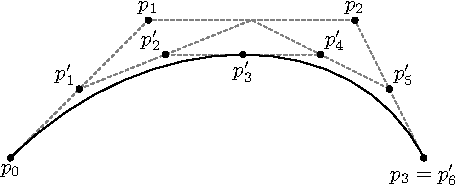
\includegraphics{subdivision}
	     \caption{A Figure Test}
	 \label{Testing Figure Label}
	\end{figure}

The image that is seen by a pinhole camera is flipped because the ray of light entering the pinhole continues through to the projection surface on the backside. Most modern cameras operate in similar fashion, where the lens acts as the pinhole. The camera body contains a sensor that detects the amount of light (or photons) that hit a certain area. Each area is representative of a pixel. In the figure above, the back plate is equivalent to the sensor. The image is not perfect, however; the use of lenses introduces various distortions, and while it is easy to imagine a ray of light entering the camera and hitting the sensor, it isn’t that easy. We need to create a model for the camera to allow us to map any object in 3D space onto a 2D image.

We have camera intrinsics and extrinsics. The intrinsics represent the various distortions and qualities intrinsic to the camera itself. The main values we care about are the focal length, FOV, and optical center, that is, the distance between the lens of the camera and the sensor, the field of view for the camera, and the pixel location for the center of the image. This allows us to take an object in 3D space and map it onto pixels in 2D space. We aren’t finished yet, because we have no frame of reference to where the camera exists in the world, these are the extrinsics. For a single camera system this is trivial, we consider the camera to be the center of the world, with no rotation issues whatsoever. When a second camera is involved, things get more complicated. In order to reconstruct a 3D location for an object given two cameras, we need to have a single origin. Otherwise we are unable to recreate all three dimensions accurately As part of the calibration process, we will take an object seen in both cameras, and figure out where the second camera is in relation to the first camera (or the center of the world). The camera extrinsics are represented in rotation and translation matrices. We will cover the calibration part later in this chapter; but the takeaway from this moment is that with these intrinsics and extrinsics that we can calculate through calibration, we can treat the cameras as a “black box” and toss in information about objects in 3D space into the appropriate matrices and the camera will spit out a corresponding image (or collection of pixels representing 3D space). More importantly, we can do this process in reverse, pointing out areas of interest on the cameras’ images, and retrieve information on where those areas are represented in 3D space.

Cameras are not perfect however. Lenses contain distortions as light travels through the lens unevenly, especially when going from the center of the lens to the edge of the lens. There are two typical distortions present in our calculations: radial distortion–often dubbed the “fisheye effect” or, inversely, the “pincushion effect”--and tangential distortion, created by a misalignment of the lens and the image plane.. This can be calibrated for, and corrected relatively easily. Lenses have three radial distortion coefficients and two tangential distortion coefficients that can be calculated during calibration and corrected thusly, 

The final modification we will make to our camera is to establish a “projection plane” for each camera (this will come up again). In short, we create a plane that is a focal length away from the lens in the opposite direction of the camera sensor. Unlike the candle example, where the resulting image is flipped, we are creating a plane for the image to appear “unflipped”. This allows us to visualize and explain higher-level concepts more simply, as we don’t have to internally flip every image we see.

\section{A (brief) Linear Algebra Primer}
Before we get too deep into the world of matrices and various transformations, it’s important to establish a baseline understanding of the calculations that are happening behind the scenes. We live in a three-dimensional world–at least that is our perception of the world. Thus, we can represent the locations of things in our world using vectors that take three values: $(X, Y, Z)$. Those values represent three different perpendicular directions. Taking those directions and scaling them accordingly, we can represent the location of anything in relation to those original directions. This can be done at home. Take your hand and create the shape of a “finger-gun” (where your index finger and thumb are both fully extended), now extend your middle finger halfway. That creates a coordinate system in terms of your fingers, and you can represent the location of objects in terms of: “how many thumbs, index fingers, and middle fingers does it take to reach an object?”

When it comes to the camera, we have two of our directions (the $X$ and $Y$ directions) that are parallel to the $X$ and $Y$ axes of the projection plane and a third direction ($Z$) which is perpendicular to the projection plane. We can then take locations represented by these vectors, and run them through our intrinsic and extrinsic matrices that define the camera to map the location onto the image. The intrinsic and extrinsic parameters of a camera can be represented with matrices. For intrinsic values, they are mapped in the following way:

We call this matrix the “camera matrix” and it is represented as $K$. Sidenote: This matrix is called “upper diagonal” which allows it some special properties that will be helpful when calibrating and mapping points.
Extrinsic parameters are commonly represented as $[R t]$, as in, the concatenated matrices of the rotation matrix (which is 3x3) and the translation matrix (which is 1x3). The resulting matrix $[R t]$ is a 3x4 matrix. With these two matrices, the equation to map a point in three-space to pixel coordinates is as follows:

Notice that the vectors representing the location in three-space and the location on the image plane contain an extra value. That is because these vectors are homogeneous coordinates. Homogeneous coordinates are representations of points in computer graphics (and in our case, photogrammetry) where perspective plays a key role. Here, the vectors take the form of $[X,Y,Z,W]$ or $[X,Y,W]$. W plays numerous roles, but its primary purpose is to aid in speedy calculations for computers by allowing translation, scaling, and rotation to be represented by matrices. An important metric of vector spaces, i.e. the three-space that we represent our three-dimensional reality in, is that the origin cannot be moved by a linear transformation, or other matrix operation. The operation of translation to a vector runs the risk of moving the origin of the vector space. If translation is the addition or subtraction of values to a vector, inputting the origin (or a vector of all zeroes) will add or subtract those values to the origin. If one tries to translate a point through clever scaling (to get around the issue of moving the origin), inputting other vectors into the same translation matrix yields wildly different results. With the introduction of a $W$ value, we can represent transformations as the following (without moving the origin).
	
\section{The Stereo Normal Example}

Triangulation is relatively straightforward if the cameras are stereo normal (the cameras are adjacent, and on the same plane of X and Z axes). In order to get to DLT, first we should cover the stereo normal base case. Cyrill Stachniss provides a great example, which I will modify for this use case.

	Imagine two cameras $O’$ and $O’’$ which share the same $Z$ and $Y$ values, pointing in the same direction (specifically the $Z$ axis), with a distance $D$ being the distance between the two cameras on the X-axis. Now, imagine a projection plane that is infinitely large, is perpendicular to the view direction to the cameras, and located a distance $F$ from the cameras on the $Z$ axis. To finish setting up, draw lines $Z’$ and $Z’’$ perpendicular to the projection plane that go through both cameras respectively. A top down view of this setup would result in the following image: 

For our stereo normal example, we are going to continue to use this view in our calculations, as we can assume any $Y$ or height information in the image will remain consistent between the two cameras (and in 3D space). This allows for a more simplistic base case, and we can elaborate on how further examples require more thought.

Now, imagine that, on the projection plane, there exists two points that map to where our blob detector has spat out the locations of the LED on each camera. Because we imagine the projection plane to be infinitely large, we map the pixel locations onto this plane using the projection, translation, and rotation matrices we were given in the initial calibration process. We will name these two points $P’$ and $P’’$ which map to cameras $O’$ and $O’’$ respectively. If we draw a line from $O’$ through $P’$ and the same for the other camera, the point at which both cameras intersect will be the location of the LED, which we will call $P$. To get that result, the math is pretty straightforward.

First, note the distance from $P’$ to $Z’$ and $P’’$ to $Z’’$ on the projection plane which we will label $x’$ and $x’’$. Through the intercept theorem, we can find the $Z$ coordinate of $P$ by solving the following relation:
\[\frac{Z}{c} = \frac{D}{-(x'' - x')}\]
Once that’s done, through Law of Similar Triangles, we can find the X coordinate of P using Z. That relation is as follows:
\[\frac{X}{x'}=\frac{Z}{c}\]
Finally, we can assume that the Y value of the coordinates is whatever the Y pixel value maps to the projection plane. This value is less important for placing the light as we can assume performers stay within the same height for this demo.

\section{Camera Calibration Process}
The camera calibration is largely done automatically through OpenCV. The method for calibrating the camera that we use is called Zhang’s method. The goal here is to gather the extrinsic and intrinsic parameters of the camera. Remember, the extrinsic and intrinsic parameters of a camera allow us to map an object in three-dimensional space onto a two-dimensional plane. To start, we want to begin with just determining the intrinsic parameters for each camera. We can assume that each camera is in the origin of their own world. The high-level explanation of this process is to choose points whose locations are known in two-dimensional space (the image) and in three-dimensional space (the world). Using that information, and the knowledge that the camera is in the origin, we can reverse engineer the camera matrix (and its parameters). However, this method is easier said than done. The current issues we face is that we want a fast way to calibrate a camera and we may not have points measured out (in three-space where the camera is the origin). We need to do some tricks.

Zhang’s method relies on the usage of a checkerboard with defined parameters; these parameters are the size of squares and the size of the grid (e.g. a 3 X 5 grid). We assume that the checkerboard is planar–or flat–on some surface. If we are able to detect the corners of the squares on the checkerboard, we could pick a single corner and know where all other corners exist in relation to it. Our first trick is setting the world coordinate system to the bottom-left corner of the checkerboard, with the $-Z$ axis being normal to the checkerboard. Then, for all corner locations on the checkerboard, they all have a single thing in common. The $Z$ coordinate of each point in three-space is 0 (or all points lie in the X/Y plane). This trick simplifies the current matrices by a significant amount. Recall that the way to convert a three-dimensional point to a two-dimensional one is as follows:
%$$\begin{matrix}{ x \\ y \\ 1} } = \begin{matrix}{ c & cs & x_H \\ 0 & c(1+m) & y_H \\ 0 & 0 & 1} \begin{matrix}{ & cs & x_H \\ 0 & c(1+m) & y_H \\ 0 & 0 & 1}\;\;\begin{matrix}{ X \\ Y \\ Z \\ 1} $$

% FIX THE MATH

Since Z = 0, we can simplify down to:
%$$\begin{matrix}{ x \\ y \\ 1} = \begin{matrix}{ c & cs & x_H \\ 0 & c(1+m) & y_H \\ 0 & 0 & 1}\left[ \matrix & cs & x_H \\ 0 & c(1+m) & y_H \\ 0 & 0 & 1} \right]\;\;\left[ \matrix{ X \\ Y \\ 1} \right]$$

During this process, we take multiple photos of the checkerboard in view of the camera. For each image we take, we find the bottom left corner of the checkerboard and establish it as the world origin. Then, knowing the size of the checkerboard squares in the real world, we generate a version of the above matrices for each corner in the checkerboard, where $K$ and $[R t]$ are the same. At this point, all we care about is what $[X, Y, 1]$ and $[x, y, 1]$ are. With that information, we can reverse engineer what K and [R t] are.

\section{DLT to 3D}
With the knowledge of the stereo normal example under our belt, alongside the knowledge of how the calibration process works, it’s time to create a non-normalized version. With the generation of projection matrices for each camera through calibration, we can theoretically take two points (one on each image), plug their location into the camera matrices, and get a point in three-space that represents the object seen in both cameras. Neither camera can output all the location information about the object on its own. A single camera can calculate the line that would intersect the object, but the second camera is needed to provide feedback on where the object is located along said line.

	One method to accomplish this is through a process called Direct Linear Transformation. At its core, it is the process of taking a matrix $Ax = w$ and minimizing $w$ (which allows us to account for noise or imperfect measurements). In this scenario, we know A is the camera matrix containing intrinsic and extrinsic parameters, and we are solving for some point $x$ such that $w$ is minimized. Note here that A is representing all the camera matrices, which is done using singular value decomposition. Essentially, the matrices that we described as the properties of the camera are in special formats that allow them to be merged into a single matrix A. Using SVD and DLT, we can take our two points on the image planes, and find a point in three-space where $w$ (or the distance between the two vectors) is minimized.

\section{From Pixels to Position}
Finally, we are in a position to cover the pipeline that exists in this project. We begin with setting up the cameras in the performance space and calibrating the cameras to the space. The program contains a calibration mode which is modified from Dr. Batpurev’s work in stereo calibration. The script takes advantage of the OpenCV library which has in-built functions to calibrate the cameras individually and as a stereo pair through Zhang’s method. We take a couple of photos for each calibration step.

Once that calibration is complete, we need to calibrate the cameras to be sensitive to only the LED that we hope to have tracked. Modern representations of images are as a matrix of three vectors, where each pixel corresponds to a set of red, green, and blue (RGB) values (sidenote, OpenCV defaults to a format of green, red, blue (GRB) values). The webcams that are used in this project operate at a resolution of 1080 pixels by 720 pixels, so to analyze a single frame of video data, the computer needs to work with 777,600 three vectors of GRB data. In order to aid the software, we want to filter out the data we don’t care about.

I used a blue LED light because it was visually distinct. That way, I can filter out pixels that don’t appear as shades of blue. This technique is called “masking”, and is pretty straightforward: First, we need to discuss a different representation of color referred to as HSV. While BGR (and other representations of RGB color) store the image as representations of the amount of red, green, and blue appear in a pixel, HSV approaches color through hue, saturation, and value. Hue represents the color, and is a value from 0-359. Colors that feature red range in the hue values of 0-60, green in the range of 60-180, blue in the range from 180-300, and back to red in the range of 300-359. The peak or most pure forms of red, green, and blue are at hues 0, 120, and 240, and allows for easy translation between RGB and HSV. Saturation represents the distance from white a color sits, and is a range from 0-100. Value is the distance from black a color sits.

HSV is actually great for image processing because it interprets color in a similar way the brain perceives color. For example, we do not see a color as a specific mix of red, green, and blue light, and when comparing two shades of the same, or similar color, we may say that one is darker or lighter, which HSV primarily encodes. In this use case, if we want to mask the image down to a certain color, we can first convert all the pixels to an HSV format, then go pixel-by-pixel, and look for pixels that fall within a certain range of hue. Because the LED light reflects off of objects, we can also filter by saturation and values to remove darker blues and focus purely on the brighter shades coming directly out of the LED.

	When we have the masked frames, the next step is to run a blob detection algorithm. The basic idea is to search the mask for blobs. A high-level description of the algorithm is to search the mask for pixels of similar color. Because the mask results in an image with only fully black or white pixels based on the hue of the LED, the light emanating from the LED results in a large clump of pixels. The blob detection algorithm allows the user to filter out blobs based on certain qualities (like the roundness of a certain blob). In our case, because we are putting so much work into filtering the image before running it through the blob detection, we allow the detector to be lenient and to flag any blobs. The detector outputs a list of all blobs it detects, specifically the image coordinates of the center of each blob. With those image coordinates, we can input into our DLT solver that we declared before. Because we calibrated the cameras, the vast majority of the work is done already. We know the camera matrix and the rotation-translation matrix for each camera, so we can input the pixel location on each camera and get a point in three-space representing the location of the LED.
	
Now that we have this location, the final step is to pick a location for the instrument and to transmit it to said instrument. Theoretically this is pretty easy. If we know the instrument’s position in relation to the world we have defined with the cameras, we can convert the location of the LED to polar coordinates. At this point, there are defined values that exist for the lighting instrument to use, and all that is left is to transmit it. I take advantage of the numerous existing python libraries that exist that allow someone to transmit a universe of data through a serial port. One of the most common serial ports that people encounter is the USB port (which stands for Universal Serial Bus). We can plug in an off-the-shelf USB to DMX decoder which–through the magic of some electronics cleverness–will output a DMX signal that runs on a five-pin DMX cable to the instrument. Rinse and repeat at least fifteen times a second and we have a functional performer tracking program!

\chapter{Bringing the Project to Life \(?\)}
The original idea was to demo the tracking software in Belle's thesis, Chronicle of a Planet. The show explores the various relationships between Belle and mother. Those representations were her own mother, her motherland as a student from China, and her mother tongue of Mandarin.

The original goal was to include the tracker in the chapter exploring motherland. In that chapter, Belle moves around a white umbrella. The intended effect was to track the umbrella in certain sections when Belle was criticizing the CCP most, to serve as the "watchful eye of a surveillance state". The show was set to open on February 14th.

\section{Where we started (this semester):}

I had ended the semester feeling a bit disheartened. At that moment I was hoping for a fully functional demo of the tracking software ready to plug into a moving light. I realize now it was a lofty task. Over that winter break, I spent some time digging around the internet to see if someone had done work with stereo vision to see what I was missing; this was when I discovered the work by Temuge Batpurev, a researcher with a PhD in Computer Science from Osaka University. Dr. Batpurev had spent time working with stereo vision, and had developed a script to calibrate stereo cameras. The issue with my project so far was that even if I had gotten a good track with the stereo cameras, the data coming out with my back-of-the-napkin math made no sense for the current context. That was because of two things: I hadn't calibrated for the distortion that a camera experiences through lenses and the fisheye effect, and I tried to rely on perfect placement of the two cameras with a measured distance instead of calibrating the two. Dr. Batpurev's script handled both of those problems.

I began the semester integrating and testing Dr. Batpurev's code. His code relies on calibrating through using a checkerboard with a specific size and row/column count. In fact, opencv provides infrastructure for detecting a checkerboard for this exact purpose (!!!). The integration proved to be fairly straightforward. The next challenge was to send instructions over DMX.

\section{DMX "Hell"}
DMX is an interesting protocol (Describe aspects of DMX and how it works as a serial protocol). While I had done some work in networking \& protocols, my knowledge of implementing it in python wasn't the greatest. Thankfully, through the magic of open-source software, there were multiple people who had created python modules designed to work in DMX transmission. One of the defining characteristics of DMX was that every packet of data to be transmitted *had* to be 513 bytes; the first one is the **start code** and it denotes the way the signal should be interpreted (usually 0x00). The other 512 bytes communicate the behavior of the following 512 addresses, with one byte assigned to each address. Because of this, the majority of open-source software I encountered would have me either create the entire 513 byte packet, or to define what addresses were needed for the light (and what data it used).

The light for this was a ROBE Esprite, provided by Outlaw Lighting--A local supplier of lighting gear. It required, on average, 49 addresses to run, to control various aspects of the light. That made for an interesting evening of starting at datasheets provided by ROBE, and using the magic of object orientation to create a consistent way to *serialize* all the attributes I needed. I ended up getting it working on its own, but I wasn't let off that easily. (Talk about the issues with USB ports \& bus space and such).

\section{So how did you get so close?}

I felt really good going into the final week before Tech (the period where all technical aspects of a show are combined). I had a way to communicate with the light, and I had a way to track the LED. Sure, I needed to still find a way to communicate the position of the LED to the Esprite, but even if I could just start to feed junk data, and just see what happens, it would have been awesome. Wishful thinking.

In order to try and speed up the tracking to be as close to real-time as possible, I downgraded the resolution from 1920x1080 to 640x480. That's a difference of 2457600 pixels to analyze to 307200 pixels (all at a hopeful speed of 20-30fps). The tracking works great when close up, but I was hoping for Belle to be dancing with the umbrella more than 15 feet from the camera, and with that resolution, the cameras had a *bit* of trouble even putting the pinprick of light that was the LED on screen. Oops.

However, if I tried to upscale the resolution, it would scale the calculations by a factor of at least 8. I am not the most efficient programmer, and some of the algorithms I used absolutely did not run in constant time (maybe elaborate on wtf that means). Even when I tried that, the computer struggled to keep pace (and also the LED did appear at a far distance very well).

Unfortunately, at that point, tech arrived and I resolved to put the project on hold while I finished designing for Belle's thesis.

\section{Where does that put us now:}

Well, it was certainly a step back, but the encouraging thing is that there is a pipeline that exists. After discussing with my advisors, the best step forward was to try to work on the pipeline in sections to figure out the capacity, and to generate demos for each particular step. That way, even if the final, full pipeline never came to completion, I would still be able to showcase my work in the various sections. The three demos Jim and I came up with were as follows:

1. [ ] A working demo showing my ability to write programmed sequences for a moving light to follow. This showcases my ability to just write onto DMX from my laptop.
2. [ ] A working demo tracking an LED with stereo camera, and displaying all the points (or points found every second) on a graph. Likely using matplotlib
3. [ ] A working demo that takes a generated graph (like one created through the previous demo), and sends it to the light.

If I can get all three working, then the pipeline should be trivial. This still means I need to work through calibrating the light, but I have some ideas on how to accomplish that. Although we are facing obstacles, this is a two step forward, one step back process.


\chapter*{Conclusion}
         \addcontentsline{toc}{chapter}{Conclusion}
	\chaptermark{Conclusion}
	\markboth{Conclusion}{Conclusion}
	\setcounter{chapter}{4}
	\setcounter{section}{0}
	
Here's a conclusion, demonstrating the use of all that manual incrementing and table of contents adding that has to happen if you use the starred form of the chapter command. The deal is, the chapter command in \LaTeX\ does a lot of things: it increments the chapter counter, it resets the section counter to zero, it puts the name of the chapter into the table of contents and the running headers, and probably some other stuff. 

So, if you remove all that stuff because you don't like it to say ``Chapter 4: Conclusion'', then you have to manually add all the things \LaTeX\ would normally do for you. Maybe someday we'll write a new chapter macro that doesn't add ``Chapter X'' to the beginning of every chapter title.

\section{More info}
And here's some other random info: the first paragraph after a chapter title or section head \emph{shouldn't be} indented, because indents are to tell the reader that you're starting a new paragraph. Since that's obvious after a chapter or section title, proper typesetting doesn't add an indent there. 


%If you feel it necessary to include an appendix, it goes here.
    \appendix
      \chapter{The First Appendix}
      \chapter{The Second Appendix, for Fun}


%This is where endnotes are supposed to go, if you have them.
%I have no idea how endnotes work with LaTeX.

  \backmatter % backmatter makes the index and bibliography appear properly in the t.o.c...

% if you're using bibtex, the next line forces every entry in the bibtex file to be included
% in your bibliography, regardless of whether or not you've cited it in the thesis.
    \nocite{*}

% Rename my bibliography to be called "Works Cited" and not "References" or ``Bibliography''
% \renewcommand{\bibname}{Works Cited}

%    \bibliographystyle{bsts/mla-good} % there are a variety of styles available; 
%  \bibliographystyle{plainnat}
% replace ``plainnat'' with the style of choice. You can refer to files in the bsts or APA 
% subfolder, e.g. 
 \bibliographystyle{APA/apa-good}  % or
 \bibliography{thesis}
 % Comment the above two lines and uncomment the next line to use biblatex-chicago.
 %\printbibliography[heading=bibintoc]

% Finally, an index would go here... but it is also optional.
\end{document}
